\chapter{Replication Strategies to Increase Storage Robustness in Decentralized P2P Architectures}
%
%
% author names and IEEE memberships
% note positions of commas and nonbreaking spaces ( ~ ) LaTeX will not break
% a structure at a ~ so this keeps an author's name from being broken across
% two lines.
% use \thanks{} to gain access to the first footnote area
% a separate \thanks must be used for each paragraph as LaTeX2e's \thanks
% was not built to handle multiple paragraphs
%
\begin{center}
Brendan~Benshoof, Andrew~Rosen, Dr.~Robert~Harrison
\end{center}



\section{Introduction}

Robustness in the face of network churn is a central issue for secure and reliable storage of data in a P2P network. 
One way to degrade a P2P network is to increase the churn rate to such  level that data is lost or the network is broken into disconnected segments. 
This paper describes a selection of strategies to increase the robustness of storage in a P2P network.
Each strategy will be described, analyzed, and finally compared and contrasted with other strategies.
We will focus on the long term efficacy of each strategy by calculating a ``half-life'' value for records in each strategy in terms of the baseline rate of churn and the number of replicas placed using the strategy.
Using half-life measurements, systems designers can consider the long term behavior of records in the network.




% If ore space needed add itemized summaries of sections

\section{Robustness}

\subsection{Robustness and Churn}
Most DHTs focus their efforts on preventing record loss due to churn.
Churn is the constant entry and exit of participants of the P2P system over time.
Established systems like Mainline DHT can see a daily net fluctuation of 10,000,000 nodes per day \cite{wang2013measuring} (about half the size of the network). 

Records are lost to churn under two conditions: the node hosting the replica leaves the network or the node with a replica ceases to be responsible for the record due to a new node joining the network and claiming that portion of the address space. 

We will describe churn as a ``Replacement ratio'': $R_{c}$, which is measured over a period of time (most often a day).
$R_{c}$ is related to the more conventional churn rate metric $\frac{exits + joins}{2 \cdot size}$ but provides more information on the volatility of records.
This value describes the portion of DHT's metric space that is maintained by a different node at the end of the period.

This is equivalent to the percentage of records that would ideally have new owners.
Ensuring these record migrate to the appropriate new owners is the primary concern of this work.  %TODO: repeat this in intro and then beat the reviewers over the head with a hammer of 


\subsection{Robustness and network partitions}
Network partitions occur when a failure results in the network separating into multiple non-connected networks.
This can be a result of failures in the underlay and the overlay networks.
The result of this is that, unlike the churn based failures,  the failure of nodes is not independent.
For example, if two previously connected regions of the Internet cease to be connected due to disaster or political intervention, there will be two new networks, each having just lost all nodes in the other partition simultaneously.
This means that robustness methods based on periodically re-storing records after they are lost are likely to be insufficient as all the possessors of a record may be found only in one of the partitions.

\subsubsection{Underlay Partitions}
An underlay partition can happen as result in a failure of infrastructure, manipulation of BGP, or governmental action.
Assuming the overlay network of the DHT has been constructed independantly of the topology underlay network, the failures due to the underlay partition will essentially occur at random locations in the network. 


While this may resemble how failure occurs during churn, the failures will all occur effectively simultaneously, to a potentially very large segment of the population of the network.
Kademlia's topology is likely to recover from such an event, however searching the network will be impaired while new connections are established.
Chord's consistent topology proof is built upon an invariant that any join or exit from the network is occurring when the majority of the network is consistent. 
The sudden failure of nodes in a underlay partition situation violates this assumption and may destroy the ability of the remaining Chord network to form a searchable overlay topology.

We will discuss underlay partitions in terms of a ratio $R_{u}$ that describes the fraction of randomly distributed members of the network that remain after an underlay partition occurs. 

\subsubsection{Overlay Partitions}
Overlay partitions occur upon the topology generated by the DHT protocol. 
In the case of an overlay partition, nodes are hypothetically able to communicate with each other but are unable to due so due to a lack of knowledge of the remainder of the network.
In practice, overlay partitions may occur due to eclipse attacks \cite{dhtsec} or logic errors in how the DHT constructs the overlay (which have been documented in the Chord protocol).
The most likely cause of an overlay partition is a result of updating a DHT protocol in a non-reverse-compatible manner, which will result in 2 non-communicating networks when only some of the participants of the network update to the new protocol.

We will discuss overlay partitions in terms of a ratio $R_{o}$ that describes the size of a connected subnetwork that remains after a partition.
It is worth considering, that in the case of any partition, the ideal behavior is that both resulting partitions remain connected, search-able, and retain discoverable replicas of all records, rather than the survival of only 1 of the partitions.

\subsection{Half Life and Time}
Traditionally in statistical discussion of databases, we consider ``Up-Time'' as the primary metric of reliability.
However in a DHT, this metric does not mesh well with reality.

Up-Time is predicated on the idea that records will never be lost, but only temporarily unavailable.
Because a DHT sees a much higher node failure rate than the data centers, where Up-Time is the primary factor of consideration, we consider any failure that would result in the temporary loss of availability of a record to simply be an increase in latency.
While DHTs attempt to minimize this latency, failure is more honestly measured in the likelihood a record will be lost forever.

Because the amount of data and rate of churn is so high, we must consider that there is a likelihood that a record can be lost simply because all of the machines that held instances of the record on the network have failed (or otherwise left the network).
With this in mind we use the metrics ``Half-Life'' and ``Mean Expected Lifetime''.

Half-Life is a unit of measure commonly used in Physics and Chemistry.
It describes the amount of time over which there is a 50\% chance that an item has ceased to exist (in the current state).
This is useful for discussing the lifetime of records in the network because we can calculate the likelihood a replica is lost due to churn over any given period of time and then use this to calculate the half life using Equation \ref{halflifeequation}.
It is important to note that the time unit for half-life is multiples of the sampling period of $R$.

\begin{equation}
\frac{-\log(2)}{\log(1-R_{period})}
\label{halflifeequation}
\end{equation}

Given an $R$ sampled in a given period, we can convert from the original period ($Period_{A}$) to a smaller or larger period ($Period_{B}$) by applying Equation \ref{eqconvert}.
This will allow us to consider the likelihood of failure over any time period where a record may be particularly vulnerable.

\begin{equation}
R_{Period_{B}}=1-(1-(R_{Period_{A}})^{\frac{Period_{B}}{Period_{A}}})
\label{eqconvert}
\end{equation}

For a single record, the half-life would represent the average expected lifetime.
For a population of replicas, the half-life would represent the period of which half of the records are expected to have been lost.
For such a population, the mean expected lifetime would describe the period required to reduce the average number of replicas to 1 (which would describe a 50\% chance of total loss).
For a population of $K$ records, the mean expected lifetime in multiples of the period of $R$ can be calculated using Equation \ref{eqlifetime}

\begin{equation}
\tau = \frac{-\log(K)}{\log(1-R_{period})}
\mbox{where $\tau$ is the lifetime.}
\label{eqlifetime}
\end{equation}


\section{Passive Replication Strategies}

Passive strategies are those where a client writes the record and replicas to the DHT once, after which no participant ever re-publishes the record.
Because of constant churn, such records are likely doomed to be lost as the nodes to which they were stored leave the network.
Because partition failures are being analyzed as specific events, rather than behavior over time, passive strategies behave the same active strategies because there will not have been sufficient time for nodes or sponsors to take action in response to the partition (if they realize a partition has occurred at all).
Passive Replication strategies are considered here primarily as a baseline of comparison for reaction to churn, and because they are identical to more active strategies in response to partition failures. 


\begin{figure}[h!]
	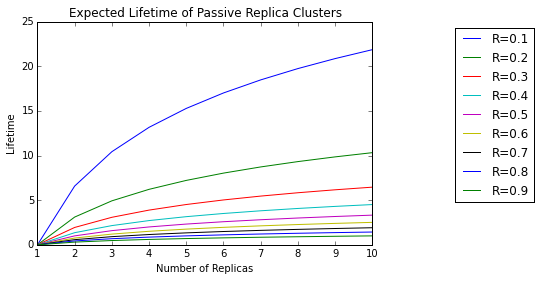
\includegraphics[width=0.5\textwidth]{figs/lifetime}
	\caption{The mean expected lifetime of a passive cluster of replicas for a given number of replicas and replacement ratios.}
\end{figure}

\subsection{$K$-Random Replicas}
The $K$-random node strategy is not used by any established DHT, however it provides a simple analytical model that we can extend to the other replica strategies.
In the $K$-random node strategy, a file is stored at $K$ locations chosen by chaining of a cryptographic hash.
That is, if a record is stored a location $L$, the first replica will be stored at location $hash(L)$ and the second at $hash(hash(L))$, etc., until $K$ nodes have been stored.

This scheme allows for simple speedup and redundancy.
Given a location $L$, any node can locate the potential $K$ backup sites and search them by order of closeness or in parallel (effectively in order of latency).
Because the locations are effectively random, we can simplify our analysis for churn and partition tolerance.

The half-life due to churn for the record (a time period over which, on average, the number of replicas in the network will be halved ) is $\frac{-\log(2)}{\log{1-R_{c}}}$.
Because the number of replicas is a small integer, we can also consider an expected mean lifetime of a record in the network: $$\frac{\log{K}}{\log(2)} \cdot \frac{-\log(2)}{\log{1-R_{c}}}$$ 
This value describes the time period after which the expected mean number of remaining replicas is 1. 
Because this 1 is the mean value, there is a 50\% likelihood there are less than 1 replica (or zero replicas, as the number of replicas is a natural number that cannot take partial values.)

This means we can present the average lifetime of a record in the network in terms of the number of replicas and churn replacement rate to be $O(\frac{-\log{K}}{\log{1-R_{c}}})$.
This implies that while more replicas always results in a longer expected lifetime, the return on adding additional replicas diminishes quickly.

The $K$-random strategy preforms similarly in both underlay and overlay partition failures (as the replicas in the network are effectively random in relation to each type of failure).
The expected fraction of surviving nodes is simply the $R$ fraction of the original network that the partition represents and the likelihood that a record is totally lost is simply the odds that all replicas are not in the considered partition: $(1-R)^{K}$. 

\begin{figure}[h!]
	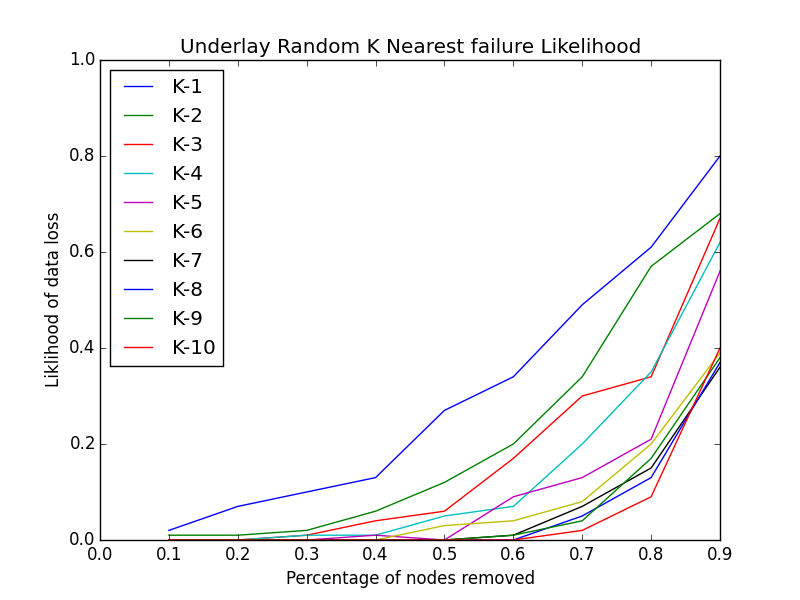
\includegraphics[width=0.5\textwidth]{figs/underlay_kad_random}
	\caption{The total loss likelihood for the k-random strategy in the Kademlia DHT with a given number of replicas and loss rate in a underlay partition scenario}
\end{figure}
\begin{figure}[h!]
	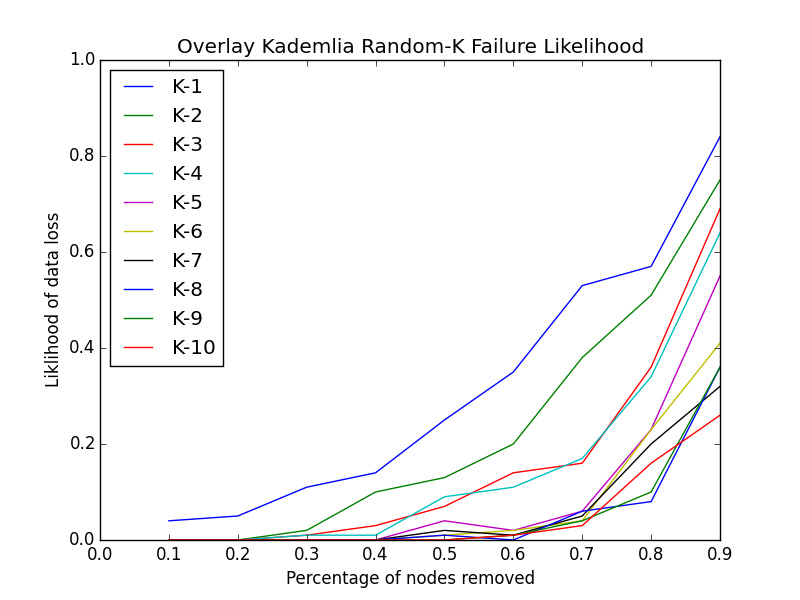
\includegraphics[width=0.5\textwidth]{figs/overlay_kad_random}
	\caption{The total loss likelihood for the k-nearest strategy in the Kademlia DHT with a given number of replicas and loss rate in a overlay partition scenario. Note that this is essentially identical to the behavior in the underlay partition failure scenario}
\end{figure}
\begin{figure}[h!]
	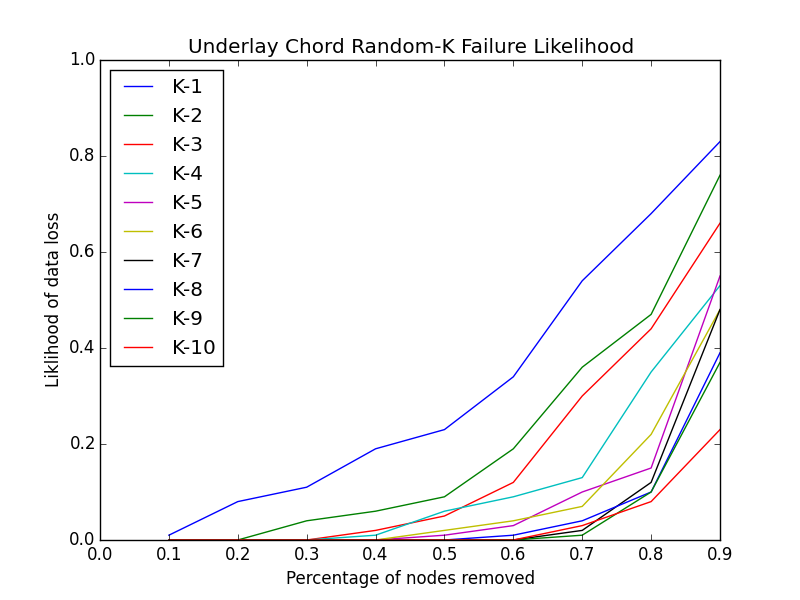
\includegraphics[width=0.5\textwidth]{figs/underlay_chord_random}
	\caption{The total loss likelihood for the k-random strategy in the Chord DHT with a given number of replicas and loss rate in a underlay partition scenario}
\end{figure}
\begin{figure}[h!]
	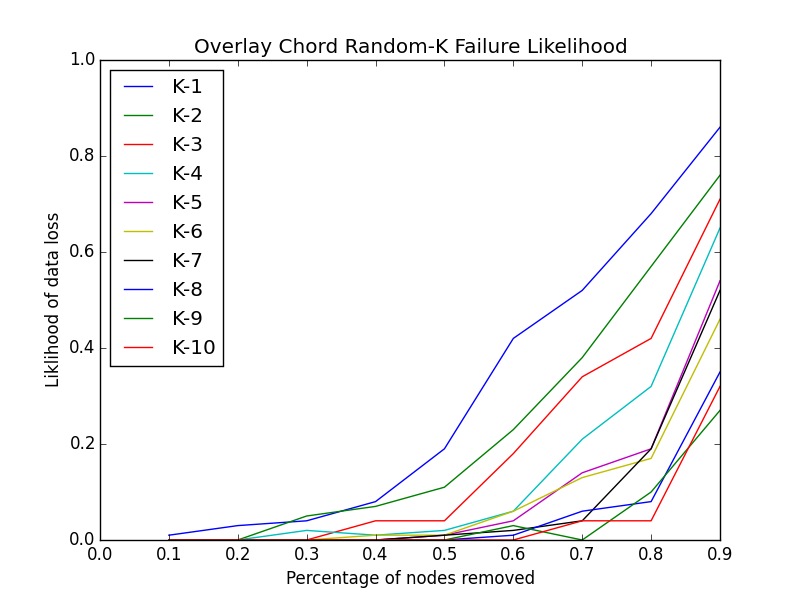
\includegraphics[width=0.5\textwidth]{figs/overlay_chord_random}
	\caption{The total loss likelihood for the k-nearest strategy in the Chord DHT with a given number of replicas and loss rate in a overlay partition scenario. Note that this is essentially identical to the behavior in the underlay partition failure scenario}
\end{figure}



\subsection{$K$-Nearest Replicas}
$K$-nearest replication is a common strategy in Kademlia based networks.
When storing a record, members preform a multi-beam search to discover the $K$ closest nodes to the target location.

This has an advantage over $K$-random nodes in that in many cases of failure, there is no downtime.
If the current owner of a record dies, an adjacent node that likely already has a backup takes over responsibility.
In terms of churn resistance and underlay failure, $K$-nearest behaves identically to $K$-random simply because the likelihood of loss due to churn is independent of the replica's location in the network.

In the case of an overlay partition, the $K$-nearest strategy is less robust because it is more likely that all the nodes in the network fall on the larger side of the partition.
Unlike the $K$-random strategy, the odds that all replicas are lost is proportional to the size of the surviving partition $R_{o}$.
This is because we can treat the entire cluster of replicas as one point because the likelihood that the cluster will be cut by the partition is negligible.
In this case, any $O(1)$ number of replicas would not provide tangible benefit.


\begin{figure}[h!]
	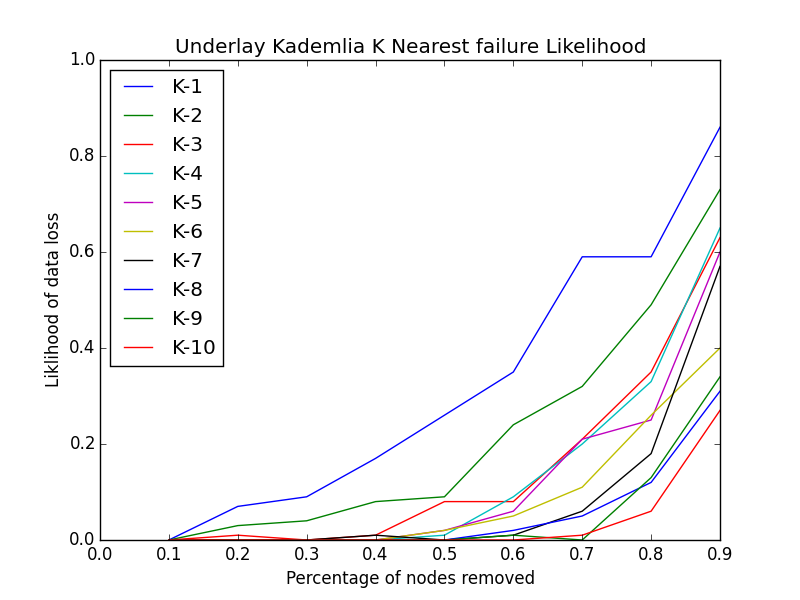
\includegraphics[width=0.5\textwidth]{figs/underlay_kad_nearest}
	\caption{The total loss likelihood for the $K$-nearest strategy in the Kademlia DHT with a given number of replicas and loss rate in a underlay partition scenario}
\end{figure}
\begin{figure}[h!]
	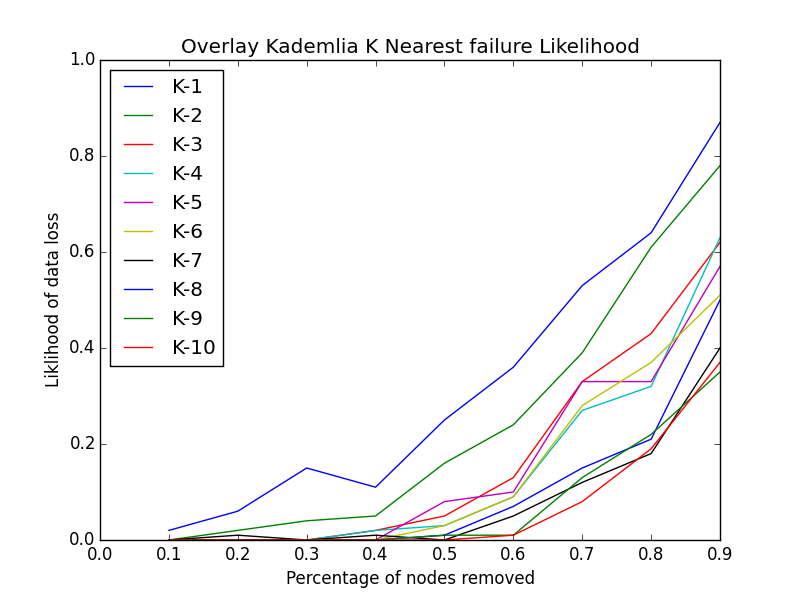
\includegraphics[width=0.5\textwidth]{figs/overlay_kad_nearest}
	\caption{The total loss likelihood for the $K$-nearest strategy in the Kademlia DHT with a given number of replicas and loss rate in a overlay partition scenario. Note that here $K$-nearest shows less reliability than in an underlay failure.}
\end{figure}
\begin{figure}[h!]
	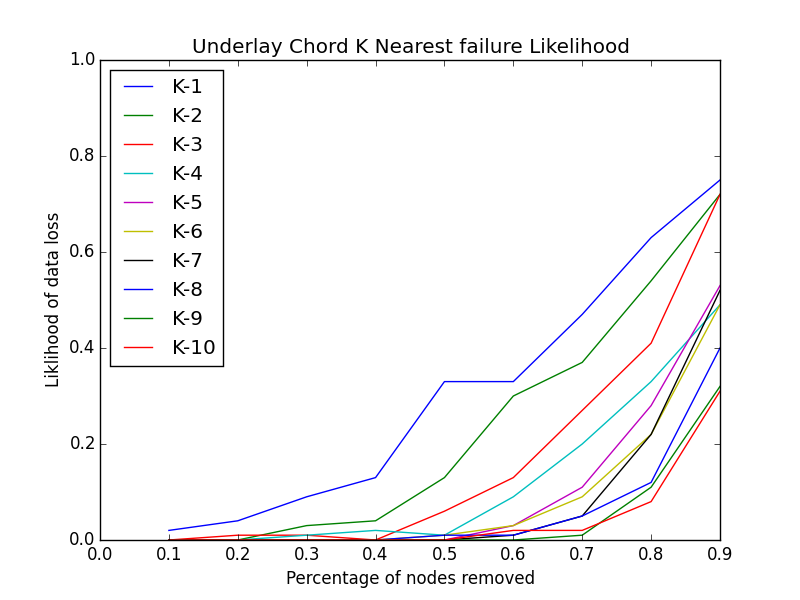
\includegraphics[width=0.5\textwidth]{figs/underlay_chord_nearest}
	\caption{The total loss likelihood for the $K$-nearest strategy in the Chord DHT with a given number of replicas and loss rate in a underlay partition scenario}
\end{figure}
\begin{figure}[h!]
	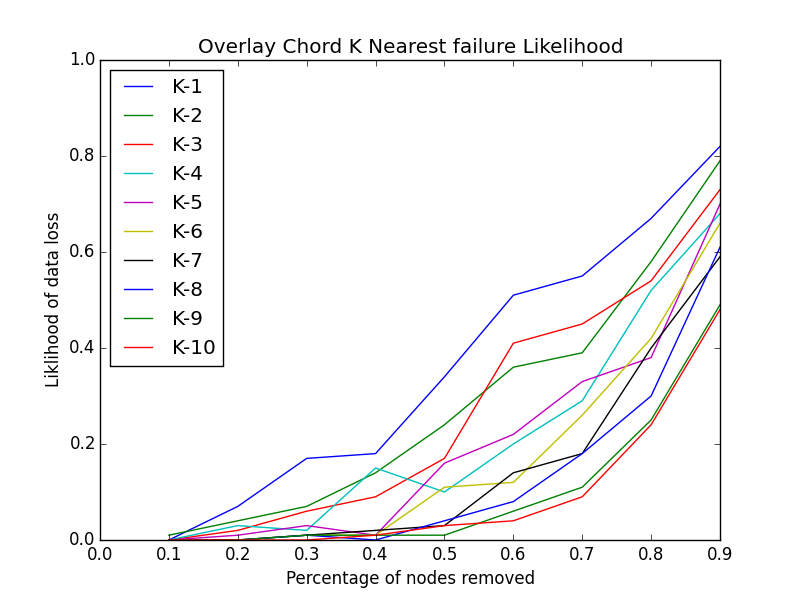
\includegraphics[width=0.5\textwidth]{figs/overlay_chord_nearest}
	\caption{The total loss likelihood for the $K$-nearest strategy in the Chord DHT with a given number of replicas and loss rate in a overlay partition scenario. Note that here $K$-nearest shows less reliability than in an underlay failure.}
\end{figure}



\section{Active Replication Strategies}

Unlike the passive replication strategies, which doomed even highly backed up records to eventual loss, active strategies result in much higher expected record lifetimes (there will always be a chance that records could be lost despite all efforts to back them up).
In active replica strategies, records and replicas are restored as they are lost due to churn.


\subsection{Active Sponsorship}

The Kademlia paper proposes a strategy for active replication \cite{kademlia}, however in practice only the ``greeting'' portion (where new nodes are given the records they are now responsible for) is implemented and Active Sponsorship is the strategy effectively used.
Rather than members of the DHT taking any actions for ensuring reliability, the DHT behaves as originally specified and acts only as dumb storage.
To ensure that a record survives churn, a sponsor outside the network periodically re-stores the record and replicas in the network.
The ideal is that this solves the problem of reliability by placing it in the hands of the users, and that critical records will have reliable sponsors.

From an analytical standpoint, the sponsor's continued ability to re-store the record is no different from the $K$-random strategy, admittedly with a much lower rate of node replacement.
Because there is no assurance that new sponsors will be created when existing sponsors are lost, Active Sponsorship only provide a higher reliability pool of nodes to be exhausted by exponential decay.
Once the sponsors have all failed, replicas will be quickly lost as discussed in passive strategies.
The half-life and expected lifetime equations of the record under active sponsorship is identical to passive strategies as we assume the lifetime provided by the higher reliability will dominate the lifetime provided by passive replication.
Some practical applications of DHTs like Bittorrent\cite{bittorrent} and IFPS \cite{benet2014ipfs} add additional sponsors as the record is demanded, however unpopular records are essentially as likely to be lost as passive $K$-random replicas once the sponsors fail.

\subsection{Active $K$-Random Replicas}
The active $K$-random  replicas strategy requires a slight modification to how the DHT stores information.
In addition to recording the key value pair, if a replica is being stored, the original location of storage must be accessible to the node.
In this strategy, all nodes in the DHT iterate over the values stored in them (likely spread out over the span of hours or a day) and ensures the record and all $k$ replicas are periodically restored.

The failure state for this strategy requires that all nodes hosting the records to be removed from the network before any one of them can restore the record.
This means, likelihood of failure over the restoration period is $R_{c}^{K}$. This essentially dramatically increases the efficacy of replicas in increasing the half-life of the record: $\tau_{1/2} = \frac{-\log{2} }{\log{(1-R_{c}^{K}})}$.
We can simplify this half-life into a format more comparable using the bound $log_{2}(1+x) \leq x$ which results in: 
\begin{equation}\tau_{1/2} \geq (\frac{1}{R_{c}})^{K}\end{equation}

Unlike the passive strategy, the addition of more replicas exponentially increases the half-life of the record in the network.
In addition, the base $\frac{1}{R_{c}}$ indicates that lowering the restoration period, and thus decreasing $R_{c}$, also causes dramatic improvements to the reliability.

Active $K$-random replicas behaves identically to passive $K$-random replicas in terms of its partition tolerance (both underlay and overlay).

In the $K$-random strategy, for each record stored with a node, that node is required to periodically communicate with $K-1$ random other nodes.
Because the number of records would far exceed the number of nodes in the network, in effect each node would be required to regularly communicate with every other node in the network.
The basic premise of the scalability of a DHT is that each node is only required to regularly communicate with a limited number of peers, so it is clear that while there are benefits to active $K$-random replication in terms of expected lifetime, the maintenance cost is prohibitive.


As an example, let us consider a network with $R_{day}$ likelihood of a record being lost per day.
If $R_{day}=0.99$ then the likelihood of loss in 1 minute is $R_{minute} = 1-(1-R_{day})^{\frac{1}{24*60}}$ or $R_{minute} = 0.0031929$. 

Given this $R_{minute}$ and the requirement for $K$ failures in the period to occur, the expected half-life of the record in the network is $\frac{-\log(2)}{\log(1-R_{minute}^{K})}$.
If $K$ is set to 10, the expected half-life in minutes of the record with 10 active replicas in a network where 99\% of the nodes are replaced in a day is $6.29  \cdot 10^{24}$ minutes or $8.7 \cdot 10^{8}$ times the age of the universe.

In practice, half-lives this large indicate that it is reasonable to expect the likelihood of the record's loss to  be dominated by partition failures and the eventual obsolescence of the network.

\begin{figure}[h!]
	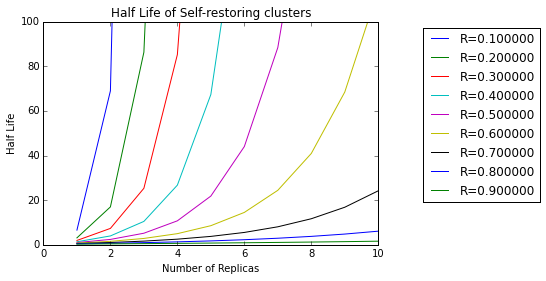
\includegraphics[width=0.5\textwidth]{figs/self_healing}
	\caption{This graph shows the expected half-life of self-rebuilding clusters of replicas in response to churn. Note that the value for R dramatically effects behavior}
\end{figure}


\subsection{Active $K$-nearest Replicas}
The basis of this strategy can be found in the Kademlia \cite{kademlia} paper, however we offer analysis and improvements that are not included in Kademlia (which offers no analysis on reliability due to the replica strategy at all).

The Active $K$-nearest replicas provides a churn robustness identical to the Active $K$-random strategy.
However it provides an opportunity for a significantly lower maintenance overhead than $K$-random replicas.
Where the random nature of backup site location effectively required the network to act as a clique, $K$-nearest associates backups with those nearby to the record.
These nodes will be the  the peers a node is already required to communicate with regularly.
This way, the number of maintenance messages is dramatically reduced to $K$ nearby peers (however the size of these messages would still be determined by the number of replicas)

\subsection{Reactive $K$-nearest Replicas}
Reactive $K$-nearest replicas is a further cost reduction on the active replication strategies, while maintaining the desired half-life of that strategy.
When replicas are associated with nearby peers, it is reasonable to expect that records will only be lost when those peers exit the network or are displaced by newly joining nodes.
Because of this, rather than attempt to track the existence of each replica, we can track the peers with which many replicas have been stored (which is already done for us by the DHT's protocol).

The means, rather than a periodic re-store of the large number of replicas, we store the replica once when the record is initially stored, and we react to the change in our peer list by re-issuing the affected records.

We can further restrict maintenance cost by limiting responsibility of re-storing of replicas to the initial owner of the record, and yet keep the same benefit of all $K$ active replicas.
We do this by giving the replica owning node the responsibility to act upon the failure of the responsible node by instantly assuming responsibility for the records closest to them (which they already have) upon the failure of the originally responsible node.

%%

%If each of the K nearest replicas is re-storing the record periodically we see an analysis similar to the Active Random K Replicas, however because nodes have more information concerning the state of nodes close to them in the network than nodes randomly located in the network.
%When a node responsible for a record fails, the replica node that assumes responsibility for the record can detect this event because it is already a peer with that node, and detection of failure is integrated into the DHT's protocol.
%This means that using only 1 responsible node to periodically restore the replicas of the record is sufficient $iff$ when the responsible node fails, the inheritor quickly detects the change in responsibility and immediately restores the K replicas (adding a new replica node to maintain K copies of the file in the network).
%This allows us to leverage the work already done by the DHT protocol to dramatically reduce both the cost of maintenance and the window of vulnerability.
%The only way for the record to be lost, is for all the replica nodes to be removed due to churn before any 1 of them detects the change in responsibility and re-publishes the records.
%It is reasonable to assume that the detection of lost peers and restoring the k-replicas can be accomplished within seconds or minutes rather than the standard 24-hour restoration cycle.


\subsection{Partition Tolerance in Active Strategies}
Active strategies do not provide improvement to handling partition failures over passive strategies
This is because, during partition failures, any active component is unlikely to be able to respond to the sudden failure.

Similarly to the passive nearest $K$ replicas strategy, the active $K$-nearest strategy is identical to $K$-random replicas in the case of an underlay partition and essentially equivalent to having no backups at all in the case of an overlay partition.
This indicates that while the active $K$-nearest strategy is incredibly robust to churn and tolerably robust to underlay failure, it is comparatively vulnerable to overlay partition failure.


\section{Experimental Validation}

For each of the strategies, we do an initial simulation of partition failures to augment formal analysis.
We simulate underlay and overlay failure on the Chord and Kademlia DHTs and report the resulting record survival rates for each strategy.
We will only consider the survival only of a single record and replicas as this simplifies computation. 
For each simulation we construct a simulated 1,000 node DHT.
We will consider underlay partitions of sizes 10\%, 20\%, 30\%, 40\%, 50\%, 60\%, 70\%, 80\%, 90\%
To simulate an underlay partition we randomly select the appropriate proportion of nodes and remove them from the topology, re-sampling each partition size with 100 trials.

Overlay partition failures are more difficult to simulate.
In order to generate a partition of a given size, we will choose a random root node, and iteratively add nodes by closeness to the root until it is of the desired size and remove the considered portion from the network. 



\section{Conclusions}

Using modifications of strategies presented in 2002 by Kademlia\cite{kademlia}, which have remained largely unimplemented for the past 14 years, we can build DHT networks that can reasonably be expected to never loose records due to churn during their active use lifetime with an overhead lower than the current actively used sponsorship based strategy.

\section{Possible Undesired Consequence of Increased Network Record Retention}

In practice, the distribution of records by age in a DHT-like network will follow an exponential distribution as older records are likely to have been lost and newer records are added.
This results in a stable ``record mass'' over time in the network as records are added at a rate similar to which they are lost.
In many ways the success of long-lived distributed hash tables seems predicated on the fact that network is unable to retain enough records to saturate storage and network capacity.

When the reactive strategy presented in this paper is implemented, there are likely to be previously unconsidered effects of node storage and network saturation if the growth rate of the network does not exceed the rate records are added.
Similarly, even if the record addition rate is low, a decrease in network size would result in the storage of the same number of replicas in less nodes, potentially saturating the capacity of the network.

